% Created 2019-02-13 Wed 13:45
% Intended LaTeX compiler: pdflatex
\documentclass[10pt]{beamer}
\usepackage[utf8]{inputenc}
\usepackage[T1]{fontenc}
\usepackage{graphicx}
\usepackage{grffile}
\usepackage{longtable}
\usepackage{wrapfig}
\usepackage{rotating}
\usepackage[normalem]{ulem}
\usepackage{amsmath}
\usepackage{textcomp}
\usepackage{amssymb}
\usepackage{capt-of}
\usepackage{hyperref}
\usepackage{minted}
\usepackage{tikz}
\definecolor{cwiRed}{HTML}{BF1238}
\definecolor{cwiBlue}{HTML}{0B5D7D}
\setbeamertemplate{footline}[text line]{%
\parbox{\linewidth}{\noindent\vspace*{2pt}\noindent\rule{\linewidth}{0.4pt}\\{\scriptsize\noindent\vspace*{7pt}\insertshortauthor\hfill\insertshorttitle\hfill\insertdate}}
}
\renewcommand*\footnoterule{}
\usepackage{lmodern}
\usetheme[progressbar=head]{metropolis}
\author{WISM454 Laboratory Class Scientific Computing, Jan-Willem Buurlage}
\date{\today}
\title{Random number generation II}
\hypersetup{
 pdfauthor={WISM454 Laboratory Class Scientific Computing, Jan-Willem Buurlage},
 pdftitle={Random number generation II},
 pdfkeywords={},
 pdfsubject={},
 pdfcreator={Emacs 26.1 (Org mode 9.1.14)}, 
 pdflang={English}}
\begin{document}

\maketitle

\section{Organization}
\label{sec:org9ac47b3}
\begin{frame}[label={sec:org6dbaf68}]{Recap}
\begin{itemize}
\item We create a reusable software library for \alert{random number generation}
\item Later in the course, we build software on top of this. We will implement libraries first for \alert{Monte Carlo methods}, and second for \alert{Genetic Algorithms}
\item Finally, we apply this generic software to some large-scale applications.
\item The reports are supposed to document this entire process!
\end{itemize}
\end{frame}
\section{RNG}
\label{sec:orgfef6b6f}
\begin{frame}[label={sec:org887fefd}]{General distributions}
\begin{itemize}
\item So far, we have focused on obtaining uniformly distributed numbers in some
set, e.g.
\begin{align*}
M &= \{ 0, 1, \ldots, m - 1 \}, \\
I &= [0, 1]
\end{align*}
\item Often, we want to draw numbers according to some other distribution function,
e.g. \alert{Gaussian}
\item There are two methods for this, that are independent on the engine used:
\begin{itemize}
\item \alert{Inversion} method
\item \alert{Rejection} method
\end{itemize}
\end{itemize}
\end{frame}
\begin{frame}[label={sec:org359bb4b}]{Random variables}
\begin{itemize}
\item Let \(\Omega\) be some \alert{sample space}, \(P\) a \alert{probability measure} on \(\Omega\).
\item Often, we will set \(\Omega = [0, 1]\), and \(P\) to be \alert{uniform probability measure}, i.e.:
$$P([a, b]) = b - a.$$
\item Random variable: a function:
$$X: \Omega \to \mathbb{R}.$$
This random variables 'realizes the desired distribution'.
\item \emph{Note:} When considering uniform distribution, we still consider a random variable \(X\) equal to the identity function (or translate-and-scale).
\item \alert{\alert{Q:}} Say you want e.g. Gaussian distribution, what to choose for \(X\)?
\end{itemize}
\end{frame}
\begin{frame}[label={sec:orgb17bbb8}]{Discrete case}
\begin{itemize}
\item Assume \(X(\Omega)\) countable, let \(x \in X(\Omega)\).
\item Discrete \alert{probability density function} (distribution function, pdf):
$$f(x) \equiv P(X = x)$$
\item \alert{Cumulative distribution function} (cdf):
$$F(x) \equiv P(X \leq x) = \sum_{t \leq x} f(t)$$
\end{itemize}
\end{frame}
\begin{frame}[label={sec:org70bcd08}]{Continuous case}
\begin{itemize}
\item Let \(X(\Omega) = \mathbb{R}\), and let \(x \in \mathbb{R}\).
\item Probability density function (pdf) or simply \alert{distribution function of \(X\)},
is the \(f: \mathbb{R} \to \mathbb{R}\) satisfying:
\begin{enumerate}
\item \(f(x) \geq 0\)
\item \(\int_{-\infty}^{\infty} f(x) dx = 1\)
\item \(\int_a^b f(x) dx = P(a \leq X \leq b)\)
\end{enumerate}
\item \alert{Cumulative distribution function} (cdf):
$$F(x) = P(X \leq x) = \int_{-\infty}^x f(y) dy.$$
\end{itemize}
\end{frame}
\begin{frame}[label={sec:orgcf64d30}]{Recap}
\begin{itemize}
\item Concepts:
\begin{itemize}
\item \alert{Random variable} \(X\)
\begin{itemize}
\item describes 'outcome of experiment' involving a random process
\end{itemize}
\item \alert{Distribution function} \(f(x)\):
\begin{itemize}
\item the probability density of observed values of \(X\) at some point \(x\)
\end{itemize}
\item \alert{Cumulative distribution function} \(F(x)\):
\begin{itemize}
\item probability of observing at most \(x\)
\end{itemize}
\end{itemize}
\item Why is this relevant to our \alert{RNG library}?
\begin{itemize}
\item Our RNGs can generate uniform numbers in \([0, 1]\).
\item We want to generate random numbers according to a \alert{specific distribution}.
\item For many distributions (Gaussian, Poisson, Binomial, \ldots{}) we know their pdf
\(f\).
\item \alert{How should we choose \(X\)} to transform our generated numbers?
\end{itemize}
\end{itemize}
\end{frame}
\begin{frame}[label={sec:orgdfe3786}]{Example: uniform distribution on \([a, b]\)}
\begin{itemize}
\item As a simple example: transform uniform distribution \([0, 1]\) to a uniform
distribution in \([a, b]\).
\item Choose:
$$X(u) = a + (b - a) u, \hspace{0.5 cm}u \in [0, 1]$$
\item Then:
$$f(x) = \begin{cases}
  0 & \text{if } x < a\\
  \frac{1}{b - a} & \text{if } a \leq x \leq b\\
  0 & \text{if } x > b
  \end{cases}.$$
$$F(x) = \begin{cases}
  0 & \text{if } x < a\\
  \frac{x - a}{b - a} & \text{if } a \leq x \leq b\\
  0 & \text{if } x > b
  \end{cases}.$$
\end{itemize}
\end{frame}
\begin{frame}[label={sec:org632c33c}]{The inversion method (idea)}
\begin{itemize}
\item \alert{\alert{Q:}} Given \(f\), find \(X\).
\item Observe that
$$u = \frac{x - a}{b - a}$$
$$u (b - a) + a = x$$
\item This is a general scheme: \alert{compute and invert the cumulative distribution}
\end{itemize}
\end{frame}
\begin{frame}[label={sec:org0b3c503}]{The inversion method}
\begin{theorem}
Let $f: \mathbb{R} \to [0, 1]$ be a distribution function with cdf $F: \mathbb{R} \to [0, 1]$.
Then $X \equiv F^{-1}: [0, 1] \to \mathbb{R}$ has distribution function $f$. 
\end{theorem}
\begin{itemize}
\item Here, the inverse \(\rightarrow\) \alert{generalized inverse}.
$$F^{-1}(u) = \text{inf} \{ x \in \mathbb{R}~|~F(x) \geq u \}.$$
\item Needed because \(F\) is not \emph{strictly} monotonically increasing.
\end{itemize}
\end{frame}
\begin{frame}[label={sec:org4cbe30f}]{Exercises}
\begin{itemize}
\item \alert{\alert{Ex 2.7}} Prove this theorem
\item \alert{\alert{Ex 2.8}} Apply to two relevant cases
\item These are hand-in exercises, hand-in a \LaTeX{}-ed solution in two weeks.
\end{itemize}
\end{frame}

\begin{frame}[label={sec:org2aa82fc}]{Limitations}
\begin{itemize}
\item Sometimes \(F\) or \(F^{-1}\) not analytically computable or even expressable
(e.g. Gaussian distribution!).
\item Instead, we can fall back to numerical methods.
\end{itemize}
\end{frame}

\begin{frame}[label={sec:org25dfdfa}]{The rejection method}
\begin{itemize}
\item \alert{Idea}: Combine two RNGs to get desired distribution
\item Let \(f\) be the desired distribution, and \(q\) some 'realizable' distribution, such that for some fixed \(c \in \mathbb{R}\):
\end{itemize}
$$\forall x \in \mathbb{R}~f(x) \leq c q(x).$$
\begin{itemize}
\item Intuitively: if we obtain a sample \(y\) according to the distribution \(q\), then the relative probability of obtaining the same sample according to \(f\) would be:
\end{itemize}
$$r \equiv \frac{f(y)}{c q(y)}.$$
\begin{itemize}
\item Sample according \(q\), then accept with probability \(r \in [0, 1]\), i.e. obtain \(u \in [0, 1]\) uniformly at random and compare with \(r\).
\end{itemize}
\end{frame}

\begin{frame}[fragile,label={sec:org22ddfbe}]{The rejection method algorithm}
 \begin{minted}[frame=none,xleftmargin=\parindent]{cpp}
auto u = lcsc::rng::uniform<double>(0.0, 1.0);
auto v = ...; // random variable with distribution q
while (true) {
    auto x = v(u.next());
    auto y = u.next();
    if (y <= (f(x) / (c * q(x)))) {
        return x;
    }
}
\end{minted}
\end{frame}

\begin{frame}[label={sec:org72cb246}]{Exercises}
\begin{itemize}
\item \alert{\alert{Ex 2.9}} (After implementing RNGs). Implement rejection method.
\item \alert{\alert{Ex 2.10}} Use RNG to generate random permutations.
\end{itemize}
\end{frame}

\begin{frame}[label={sec:orga7d73e1}]{High-level overview of RNG library}
\begin{center}
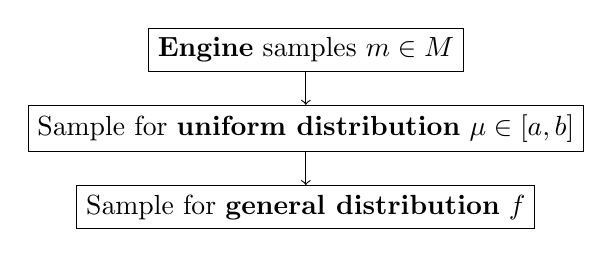
\begin{tikzpicture}
\node[draw] (a) {\textbf{Engine} samples $m \in M$};
\node[draw, below of=a] (b) {Sample for \textbf{uniform distribution} $\mu \in [a, b]$};
\node[draw, below of=b] (c) {Sample for \textbf{general distribution} $f$};

\draw[->] (a) -- (b);
\draw[->] (b) -- (c);
\end{tikzpicture}
\end{center}

\begin{itemize}
\item Arrows are independent of specific methods!
\end{itemize}
\end{frame}
\section{C++}
\label{sec:org73576f0}
\begin{frame}[label={sec:orgbbfdf2d}]{Second tour of C++}
\begin{itemize}
\item We continue with our overview of the C++ language
\item I don't expect you to become a fluent C++ programmer by only looking at these
slides!
\item Consider the C++ lectures as a \alert{summary of topics} that you are supposed to
familiarize yourself during this course
\item Learning C++ is best done by consulting references (and writing a lot of
code)!
\begin{itemize}
\item \emph{Bjarne Stroustrop} - The C++ Programming Language
\item \emph{Scott Meyers} - Effective Modern C++
\item \url{https://en.cppreference.com}
\item \ldots{}
\end{itemize}
\end{itemize}
\end{frame}
\begin{frame}[fragile,label={sec:org7350acd}]{Arrays and pointers (I)}
 \begin{itemize}
\item Recap:
\end{itemize}

\begin{minted}[frame=none,xleftmargin=\parindent]{cpp}
int xs[5] = {1, 2, 3, 4, 5};  // array of integers 
int x = xs[3]; // x is now 4
int* p = &xs[3]; // pointer to 3rd element of xs
std::cout << p << "\n"; // ~> "0x1a2b3c4d"
std::cout << *p << "\n"; // ~> "4"!

++p; // increase pointer (not value)
std::cout << *p << "\n"; // ~> "5"!
\end{minted}

\begin{itemize}
\item Operator \texttt{\&}: \alert{address of}
\item Operator \texttt{*}: \alert{contents of} (also called dereferencing).
\end{itemize}
\end{frame}
\begin{frame}[fragile,label={sec:orgb83d1ef}]{Arrays and pointers (II)}
 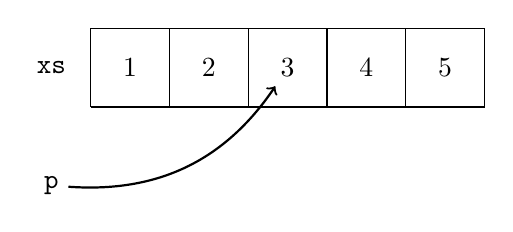
\begin{tikzpicture}
\draw (0,0) grid (5,1);
\node at (0.5, 0.5) {1};
\node at (1.5, 0.5) {2};
\node (3) at (2.5, 0.5) {3};
\node at (3.5, 0.5) {4};
\node at (4.5, 0.5) {5};
\node at (-0.5, 0.5) {\texttt{xs}};

\node (p) at (-0.5, -1.0) {\texttt{p}};

\draw[->, thick] (p) edge[bend right] node {} (3);
\end{tikzpicture}

\begin{itemize}
\item \texttt{xs} is the array containing data (stored as a pointer to the first element)
\item \texttt{p} is free to point to any element, i.e. \texttt{p = xs} would make \texttt{p} point to the
first element!
\item Dealing with pointers is tricky business! In modern C++, they are avoided
wherever possible.
\end{itemize}
\end{frame}

\begin{frame}[fragile,label={sec:org8905c32}]{References}
 \begin{minted}[frame=none,xleftmargin=\parindent]{cpp}
int x = 3;
int& y = x;
y = 4;
std::cout << x << "\n"; // ~> "4"

void f(int x, int& z) {
    z = x * x;
}

int z = 0;
f(x, z);
std::cout << z << "\n"; // ~> "9"
\end{minted}

\begin{itemize}
\item A reference is like a pointer, but need not be dereferenced explicitely.
\item It is like an alias, can only be initialized once
\item Prefered over pointers
\end{itemize}
\end{frame}

\begin{frame}[fragile,label={sec:org10baf73}]{\texttt{const}-ness}
 \begin{minted}[frame=none,xleftmargin=\parindent]{cpp}
const int x = 3;
x = 5; // ERROR

int f(const int& x) {
    return x * x;
}
\end{minted}

\begin{itemize}
\item A promise not to change a value, but merely use it
\item In this case, we don't copy the \texttt{int}, but share a reference to it
\item Important part of an interface!
\end{itemize}
\end{frame}

\begin{frame}[fragile,label={sec:org20f956a}]{Stack vs Heap memory}
 \begin{itemize}
\item A big motivation for using pointers is the difference between stack and heap
memory.
\end{itemize}

\begin{minted}[frame=none,xleftmargin=\parindent]{cpp}
int x = 3; // integer allocated on the stack

int* x = new int; // integer allocated on the heap
*x = 3;
delete x;
\end{minted}

\begin{itemize}
\item Default: put on the stack. Limited space available. Automatically 'deallocates' when out of scope.
\item Heap slower, but bigger and more flexible (dynamic deallocation)
\end{itemize}
\end{frame}

\begin{frame}[fragile,label={sec:org9e8feb1}]{Dangling pointers and references}
 \begin{itemize}
\item \emph{Dangling pointers}: pointer to objects that are not valid.
\end{itemize}
\begin{minted}[frame=none,xleftmargin=\parindent]{cpp}
// references to objects that have gone out of scope
int& f() {
  int c = 3;
  return c;
}

auto& x = f();

// 'use after delete'
auto i = new int;
*i = 3;
auto j = i;
delete i;
std::cout << *j << "\n";
\end{minted}
\end{frame}
\begin{frame}[fragile,label={sec:orgcdcfc5d}]{Classes and other user-defined types}
 \begin{itemize}
\item So far, we have only looked at \alert{built-in types}
\item New types can be created in two main ways, by \alert{classes} and \alert{enumerations}.
\item Writing software for C++ is mostly about defining your own types, and
operations on them! Simplest example is the \texttt{struct} from C
\end{itemize}

\begin{minted}[frame=none,xleftmargin=\parindent]{cpp}
struct lcrng {
    int a;
    int c;
    int m;
};
\end{minted}

\begin{itemize}
\item A LCRNG is defined by the three numbers \(a, c, m\), it makes sense to define a
type that groups them together.
\end{itemize}
\end{frame}

\begin{frame}[fragile,label={sec:orgf22af78}]{Classes (II)}
 \begin{minted}[frame=none,xleftmargin=\parindent]{cpp}
lcrng r;
r.a = 14239;
r.c = 5205;
r.m = (1 << 30) - 1;

int next(lcrng r, int x) {
    return (r.a * x + r.c) % r.m;
}

auto seed = 12345;
auto x1 = next(r, seed);
\end{minted}
\end{frame}

\begin{frame}[fragile,label={sec:orgebc6744}]{Classes (III)}
 \begin{minted}[frame=none,xleftmargin=\parindent]{cpp}
// alternative initialization
lcrng r = {14239, 5205, (1 << 30) - 1};
auto r = lcrng{14239, 5205, (1 << 30) - 1};

// *member* function 
struct lcrng {
    int next(int x_prev) {
        return ...;
    }

    int a;
    int c;
    int m;
};
\end{minted}
\end{frame}

\begin{frame}[fragile,label={sec:orge1d28f4}]{Classes (IV)}
 \begin{minted}[frame=none,xleftmargin=\parindent]{cpp}
class lcrng {
  public:
    lcrng(int a, int c, int m, int seed) :
        a_(a), c_(c), m_(m), x_(seed) {}

    int next() {
        return ...;
    }

  private:
    int a_;
    int c_;
    int m_;
    int x_;
};
\end{minted}
\end{frame}

\begin{frame}[fragile,label={sec:orgf792fca}]{Classes (V)}
 \begin{minted}[frame=none,xleftmargin=\parindent]{cpp}
auto park_miller = lcrng(16807, 0, (1 << 31) - 1), seed);
for (int i = 0; i < samples; ++i) {
    std::cout << park_miller.next() << "\n";
}
\end{minted}
\begin{itemize}
\item Note that when we are given \texttt{park\_miller}, we can generate random numbers
simply by calling \texttt{next} on it.
\end{itemize}
\end{frame}

\begin{frame}[fragile,label={sec:org635c15e}]{Polymorphism}
 \begin{itemize}
\item Another important application of references/pointers
\end{itemize}

\begin{minted}[frame=none,xleftmargin=\parindent]{cpp}
class rng {
  public:
    virtual int next() = 0;
};
\end{minted}

\begin{itemize}
\item An RNG is anything implementing \texttt{next}..
\end{itemize}

\begin{minted}[frame=none,xleftmargin=\parindent]{cpp}
class lcrng : public rng {
    ...
    int next() override {
        return ...;
    }
    ...
};
\end{minted}
\end{frame}

\begin{frame}[fragile,label={sec:org9358df0}]{Polymorphism (II)}
 \begin{itemize}
\item In many cases (e.g. obtaining real uniform distribution from integer one), we
do not care about the specific engine!
\end{itemize}

\begin{minted}[frame=none,xleftmargin=\parindent]{cpp}
class uniform_real_distribution {
  public:
    uniform_real_distribution(const rng& engine) { ... }

    float sample() { ... }
}
\end{minted}

\begin{itemize}
\item This is an example of polymorphism!
\end{itemize}
\end{frame}

\begin{frame}[fragile,label={sec:org8eb7331}]{Namespaces}
 \begin{itemize}
\item Group your functions and types together under a single 'namespace', e.g.:
\end{itemize}

\begin{minted}[frame=none,xleftmargin=\parindent]{cpp}
namespace lcsc {

class rng { ... };
void plot_histogram(const rng& engine) { ... }

} // namespace lcsc

lcsc::plot_histogram(lcsc::lcrng(...));
\end{minted}
\end{frame}

\begin{frame}[fragile,label={sec:orgfa07146}]{Summary}
 \begin{itemize}
\item Today we covered
\begin{itemize}
\item arrays, pointers and references
\item \texttt{const} and its applications
\item stack versus heap memory
\item classes and structs
\item polymorphism
\item namespaces
\end{itemize}
\item Over the next couple of weeks, we will apply all of these concepts to write a RNG library that we
will use throughout the course.
\item Example structure and interface available on the course website
\item Strongly suggest to design your own interface!
\end{itemize}
\end{frame}
\section{Tutorial}
\label{sec:org912c618}
\begin{frame}[label={sec:orga757dfd}]{This week}
\begin{itemize}
\item Tutorial:
\begin{itemize}
\item Demo of compiling with multiple files, see GitHub course page
\item Set up RNG structure with classes
\item Implement number of LCRNGs in this new system
\item \alert{Ex 2.9} (rejection method)
\item \alert{Ex 2.10} (random permutations)
\end{itemize}
\item At home (hand-in exercises):
\begin{itemize}
\item \alert{\alert{Ex 2.7}} Prove \emph{inversion of cdf} theorem
\item \alert{\alert{Ex 2.8}} Apply to two relevant cases
\end{itemize}
\end{itemize}
\end{frame}
\end{document}